\section*{Pipeline}
All configurations are done in the config.toml file. It begins with
%
\begin{lstlisting}
# TOML for XenSegEval
[owner]
name = 'Normann-BPh'
mail = 'philomina-lillie.normann@bih-charite.de'

[Tasks]
preprocess = false
segment = false
evaluate = true
\end{lstlisting}
the owner variable is not relevant for the pipeline. 'mail' is used to send SLURM updates to. if the pipeline is run as is, then it requires a SLURM server. information on start, fail, end and time constraints are sent to the mail. \\
The subprocesses 'preprocess', 'segment', 'evaluate' are only started if the value is set to 'true'.
it continues with
\begin{lstlisting}
[paths]
# directory the processed data will be saved to
# as default this will be the cloned directory
home = 'drive/group/user/home'
# directory of Xenium-results
data_path = '(home)/xenium_output'
# give a name to the sample
sample_name = 'TMA[X]'
# path to ground_truth
gt_path = '(home)/clone/ground_truth.tif'
# path to the user-defined section
# one must have the same coordinates
# as the gt-masks
sections_path = "(home)/clone/section.json"
\end{lstlisting}
(mostly) all paths above are required to be defined before starting the pipeline. 'home' defines the directory where the output - images \& transcripts, segments, evaluation, logs - will be saved. 'data\us path' is the directory containing the Xenium output as defined above. 'sample\us name' the name to give the sample run, example: TMA1 for tissue microarray 1. 'gt\us path' the path to the groundtruth masks. required if evaluation based on Jaccard and co is used. 'sections\us path' the path to a json file of the section to evaluate on. required if running any evaluation. the provided ground truth must have the coordinates in sections\us path.\\
the Image has stats that are better provided, or verified, before the pipeline.
\begin{lstlisting}
[ImageStats]
# stats of the morphology.ome.tif
# micrometer per pixel
pixelsize_xy = 0.2125
pixelsize_z = 3.0000
# resolution
y = 64612
x = 51096
\end{lstlisting}
width and height of the image (x,y) mustn't be provided. pixelsizes should be checked before and corrected if necessary.\\
config for the SLURM nodes
\begin{lstlisting}
[sbatch]
# sbatch job specifications
gpu = "gpu:l40:1"
# time in days
time = 2
# RAM in gigabyte
mem = 64
# nr. cores
cpu = 20
\end{lstlisting}
all, except ProSeg, require a gpu to work efficiently and to provide results comparable to those presented here. the variable must be exactly as the server requires the definition. for the BIH HPC cluster it's defined as above, gpu:abbreviation:amount. the pipeline runs on a 1.2K x 1.7K image for roughly an hour and a half, for safety each node is started with a 2day time limit. some processes, especially ProSeg and image preprocessing, need high RAM. many processes are parallelized using pythons multiprocessing, right amounts of cores can speedup the processes. currently the most cores are required by the cross evaluation, one core for each output = 15 cores. \\
to process the morphology image as needed configure the part below
\begin{lstlisting}
[preprocessing]
# layers user is interested in
# leave list empty if only
# multi-layer required
planes = [5, 6, 7]
# number of expected sections
n_roi = 12
# additional space around the roi
buffer = 0.01
# number of chunks a section is 
# split into for faster processing
# set to zero for None
# must be 0,4,9,16,25,...
chunks = 4
# overlap of chunks in percent
overlap = 0.05
\end{lstlisting}
the preprocessing prepares three datasets. the images, which are morphology and focus split into the detected (n\us roi tells the pipeline how many regions of interes, how many punches, are expected), or provided, punches, each sample in a separate folder, morphology additionally separated into chunks and layers (the layers in all images are defined by the 'planes' variable). the transcipts also split into separate files, each containing the measured transcripts in the punch region, converted into pixel coordinates, relative to the sections origin. the same is done to the xenium provided boundaries of cells and nuclei. \\
'buffer' adds few more pixels around the preliminary defined section. if the sections are expected to be very large, or have a lot of layers important for the segmentation, then the user can provide a number of chunks to split the images into. must be an integer square-root. the overlap between the chunks is defined by 'overlap' on percentage. \\
what follows then are the model specific parameters. please consult the documentation of the repsective model. a good start is the model or wrapper definition, they are provided in the default config file at the begining of each parameter-table.\\
to configure the evaluation, modify the variables under '[evaluation]'
\begin{lstlisting}
[evaluation]
# if a evaluation should be performed based on
# Jaccard and related scores
[evaluation.jaccard]
use = false

# Jaccard but by cs-benchmark
[evaluation.cs_bench]
use = false

# not implemented yet
	# principal components
	[evaluation.pca]
	use = true
	
	# probability density
	[evaluation.pd]
	use = false
	overlay_image = false

[evaluation.cross]
use = false
# 'cs' or 'af1'
benchmark = 'af1'
# choose metric according to benchmark
metric = 'Jaccard'
# relevant for 'af1'
threshold = 0.5
\end{lstlisting}
%
\begin{figure}
    \centering
    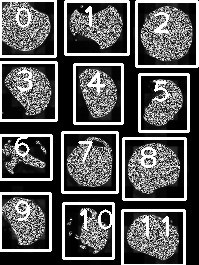
\includegraphics[width=0.5\linewidth]{Images/marked_regions-of-interest.png}
    \caption{Regions marked automatically by the pipeline if no section is given.}
    \label{fig:mROIs}
\end{figure}
% 
rsatoin
% 
\vspace{8pt}
\begin{figure}
    \label{fig:directory structure}
    \dirtree{%
        .1 \textless smaple name\textgreater.
        .2 processed.
        .3 \textless section\textgreater.
        .4 boundaries.
        .5 cell\us relative.parquet.
        .5 nucleus\us relative.parquet.
        .4 morphology.
        .5 focus.
        .6 focus.ome.tif.
        .6 quartered.
        .7 q0\%c.ome.tif.
        .5 multi\us layer.
        .6 morphology.ome.tif.
        .6 quartered.
        .7 q0\%c.ome.tif.
        .5 single\us layer.
        .6 layer0\%L.
        .7 morphology.tif.
        .7 quatered.
        .8 q0\%c.tif.
        .4 transcripts.
        .5 relative.csv.gz.
        .5 relative.parquet.
        .3 marked\us regions-of-interest.tif.
        .3 sections\us px.json.
        .2 results.
        .3 \textless method\textgreater.
        .4 evaluation.
        .5 \textless section\textgreater.
        .6 layer.
        .7 CS-BENCH.csv.
        .7 false\us negatives.csv.
        .7 results.csv.
        .7 split\us merges.csv.
        .4 output.
        .5 \textless section\textgreater.
        .6 \textless ...\textgreater.
        .2 run.
        .3 jobs.
        .4 \textless method\textgreater.sh.
        .3 logs.
        .4 \textless method\textgreater\us \%N\us \%j.err.
        .4 \textless method\textgreater\us \%N\us \%j.out.
    }
\end{figure}